\chapter{Survey}
\label{chp:amtsurvey} 

\section{Constructing the Survey}

\subsection{How and why we chose this design}
%hvorfor vi satte spørsmålene der vi gjorde osv osv. Design!
%Hvorfor surveymonkey?
%hvordan vi gikk fram på AMT? hvorfor amt?

\section{Survey Results}
%Hvor mange svar vi fikk og sånn
%Hvordan vi har gått gjennom resultatene, hva vi har fokusert på og hvorfor!

\subsection{Demographics}
As mentioned before we distributed our survey on two platforms; Amazon Mechanical Turk (AMT) and Facebook. As you can see in \fref{fig:land}, the distribution was mainly divided between two countries, the United States of America and Norway. Other countries are also represented; Canada, France, Germany, India, Indonesia, Ireland, Jamaica, Romania, Russia, Serbia and United Kingdom. 77 of the 250 responses were collected through the Facebook link, and out of these 77 people 96\% (74 people) are from Norway. 173 of the 250 respondents took the survey via Amazon Mechanical Turk, and out of these people 85,5\% (148 people) are from the United Stated of America. 

\paragraph{}
The majority of the total respondents were female. They accounted for 56,80\% of the responses, which is 142 responses. This means that 43,20\% of the total respondents were male, with a 108 responses. We saw a difference in the gender distribution from the Facebook link and from AMT. On AMT 38,15\% were men, and 56,80\% were female. On Facebook 54,55\% were male, and 45,55\% were female. In other word the majority of respondents on AMT were females, in contrary to Facebook, were the majority of respondents were men. The different gender distributions are shown in the \fref{fig:gender}.
 
\begin{figure}[h!]
\centering
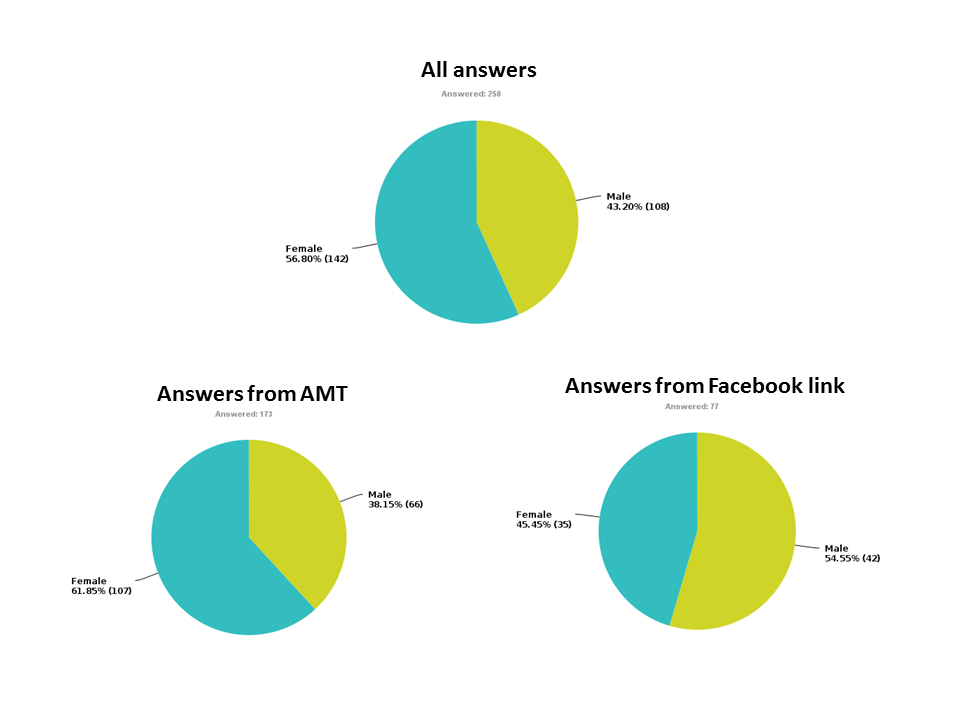
\includegraphics[width=1\textwidth]{gender.png}
\caption[Gender distribution]{\textbf{Gender distribution}. This graph shows the overall gender distribution (on the top), gender distribution from AMT (to the left) and the gender distribution from the Facebook link (to the right).} 
\label{fig:gender}
\end{figure}

\paragraph{}
Among the participants the age ranged betweetn 19 and 76. The average age is 31. The average age of the AMT participants (33 years old) are higher than the average age of the Facebook participants (27 years old). When we look at the total income of the household per year and employment status, we find a wide range of variety among the participants. We have several participants in each group of income. Although the majority of the participants are employed for wages or students, all of the other employment status' are represented. This is consistent with former studies of AMT users \cite{incentivesAmt}. 

\begin{figure}[h!]
\centering
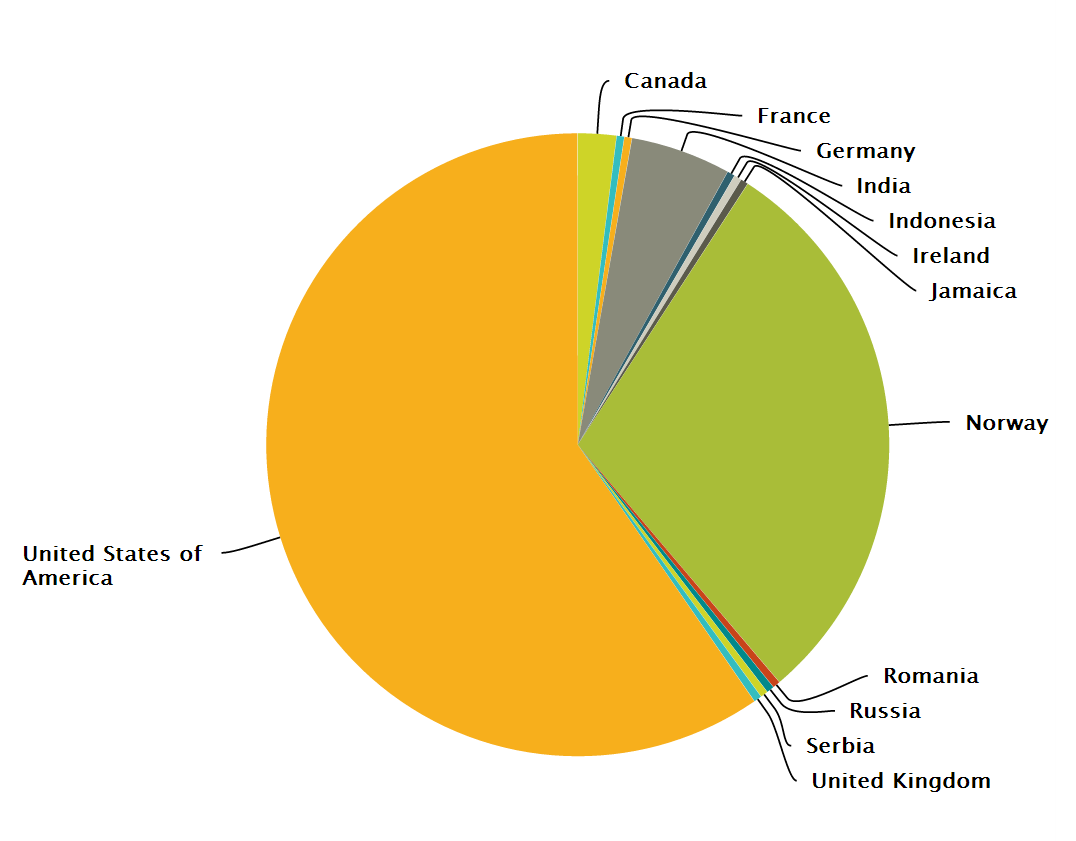
\includegraphics[width=1\textwidth]{land.png}
\caption[Distribution of the participant's country of origin]{\textbf{Distribution of the participant's country of origin}. This graph shows the distribution of the participant's country of origin. Most of the participants are from the United Stated of America and Norway.} 
\label{fig:land}
\end{figure}

\subsection{Never Checked Facebook Privacy Settings During the Last Year}
% De som svarte "never checked" på Q3
30 of the people who answered our survey stated that they have never checked their privacy settings during the last year. Even though they have not checked the privacy settings during the last year, most of them have done some changes to their settings before the previous year. 

Average number of friends: 162
Average age: 39

\begin{figure}[h!]
\centering
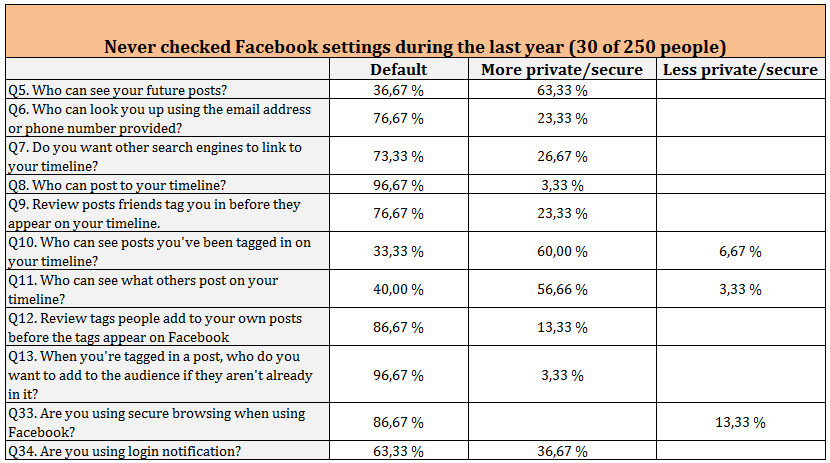
\includegraphics[width=1\textwidth]{nevercheckedtable.png}
\caption[Bilde 1]{Bilde 11} 
\label{fig:co}
\end{figure}

60\% did not consider changing privacy settings after reviewing them. 
40\% wanted to make their privacy settings more private. 

Quote from \#2 on Question 23: "Now you have scared me. I am alone and afraid" -Random Female with Ph.D, 5 friends and 67 years old. 

For example under "Who can see your future posts?" 11 people answered public and 19 persons answered friends.
- Default is public

On the setting "Who can look me up? Do you want other search engines to link to your timeline?" 22 has it on (this is default), and 8 has turned it off. 

7 of them has enabled the "Review posts friends tag you in before they appear on your timeline". 

\subsection{Checks Privacy Settings "Once a month" or "Once a week or more"}
Average number of friends: 416
Average age: 28,5

85\% of these people checks their Facebook at least once a day.
70,83 \% did not consider changing privacy settings after reviewing them. 
27,08 \% wanted to make their privacy settings more private.
2,08\% considered changing them to more public 

12 of the 48 people in this category answered yes on the question whether or not facebook had affected their personal life negativally. Half of these had situations with friends posting unwanted pictures (av forskjellige grunner) of them.

One guy: Two accounts; one under a pseudonym for friends only and on with strict settings for the rest of the world. "Privacy is important to me. It is meaningless not to give others the same courtesy" - Random guy with 420 friends that are 43 years old. 

\begin{figure}[h!]
\centering
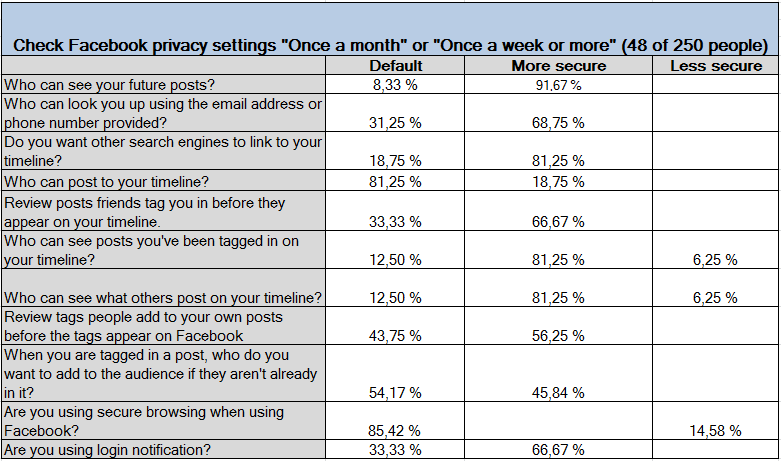
\includegraphics[width=1\textwidth]{checkonceaweekormoretable.png}
\caption[Bilde 1]{Bilde 11} 
\label{fig:co}
\end{figure}

\subsection{Interdependent Privacy}


